\section{Implementation}
During the implementation phase, we encounter several challenges due to integration issues,
as well as in our developmental workflow. We constantly iterated and tried new approaches.
Our three main approaches that worked to product a functional OCR are outlined below.

\subsubsection{Native Android App - OpenCV}
We initially attempted to implement a native android application, using the Java Native Interface
to run OpenCV C++ code. However, we were quickly bogged down by dependency and programming environmental
issues. After a painstaking week of debugging, we realized that due to the android platform, we would
not be able to run both JavaCV and native OpenCV in the same application - an error was thrown about
a duplicate in the .apk file. \\
Nevertheless, we were able to get a quick prototype up and running.
The code can be found in the 18551\_Prototype android project. We were able to get a touch-based
selection box working. As a prototype, we also managed to linked tesseract - Google's Open Source OCR Engine - 
to our application giving us decent OCR capabilities. These were done through different Views and Touchevents.\\

However, as mentioned there were integration issues,
and we decided to move the project fully onto JavaCV, rationale being that we had only one member - James - 
that was knowledgeable about C/C++, and in this way more team members could contribute.

\subsubsection{Android App - JavaCV}
\begin{figure}[h]
	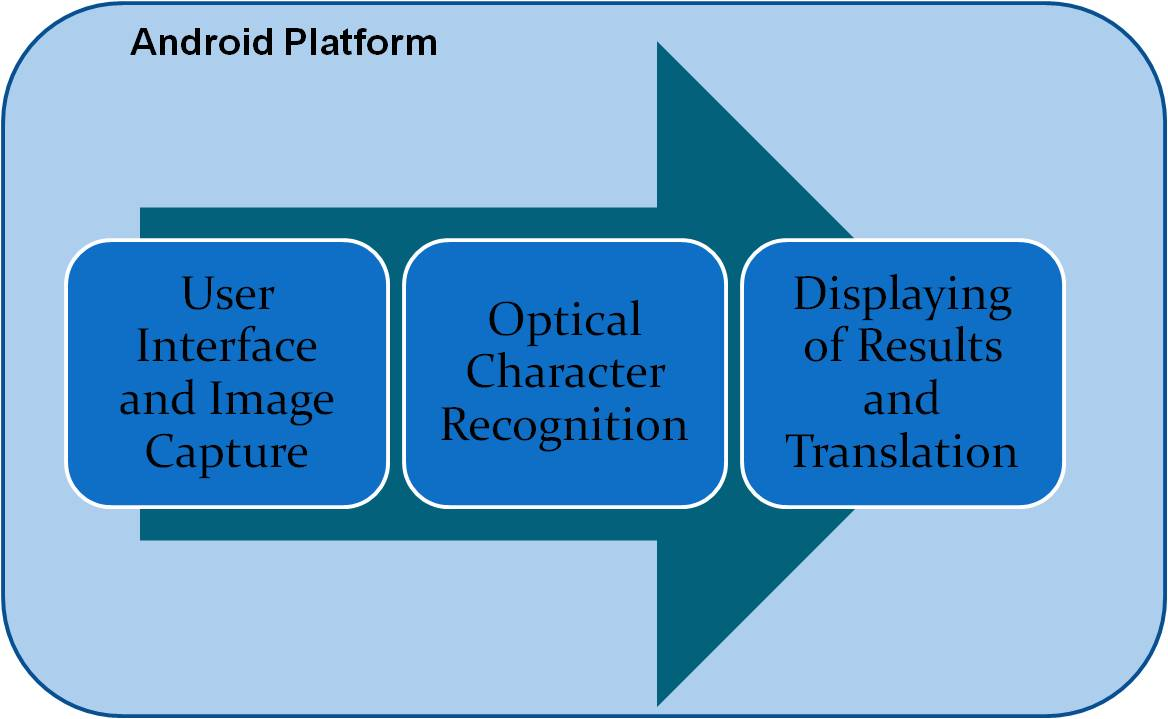
\includegraphics[scale=0.75]{androidFramework.jpg}\\
	\caption{Framework for Android JavaCV App}
	\label{fig:androidFramework}
\end{figure}
Figure \ref{fig:androidFramework}  shows our framework for the Android JavaCV App. After the initial integration issues
with the native Android App, we transitioned over to a pure JavaCV application. As shown, everything occurs
on the Android platform itself. Naturally, however, this had its drawbacks, namely being cumbersome to iteratively
develop on. Loading of android application (apk) files were slow - it could take up to 30 seconds to compile, upload
and install the application on the device. The Android platform itself also had a limited amount of memory, and
was unable to handle more than 3 large bitmaps (i.e. 1592 x 2944 size) bitmaps at a time, which slowed our debugging
process. Processing speed was also much slower than in Matlab on a laptop - early implementations took ~14 seconds to
pre-process the image. Finally, little documentation for Java OpenCV functions existed, slowing progress. Due to these
conditions, and the fact that one of our team members was only fluent in Matlab, spurred us to create another framework
for debugging and development. The code can be found in the 18551\_Project android project.

\subsubsection{Android Client Server Model}
\begin{figure}[h]
	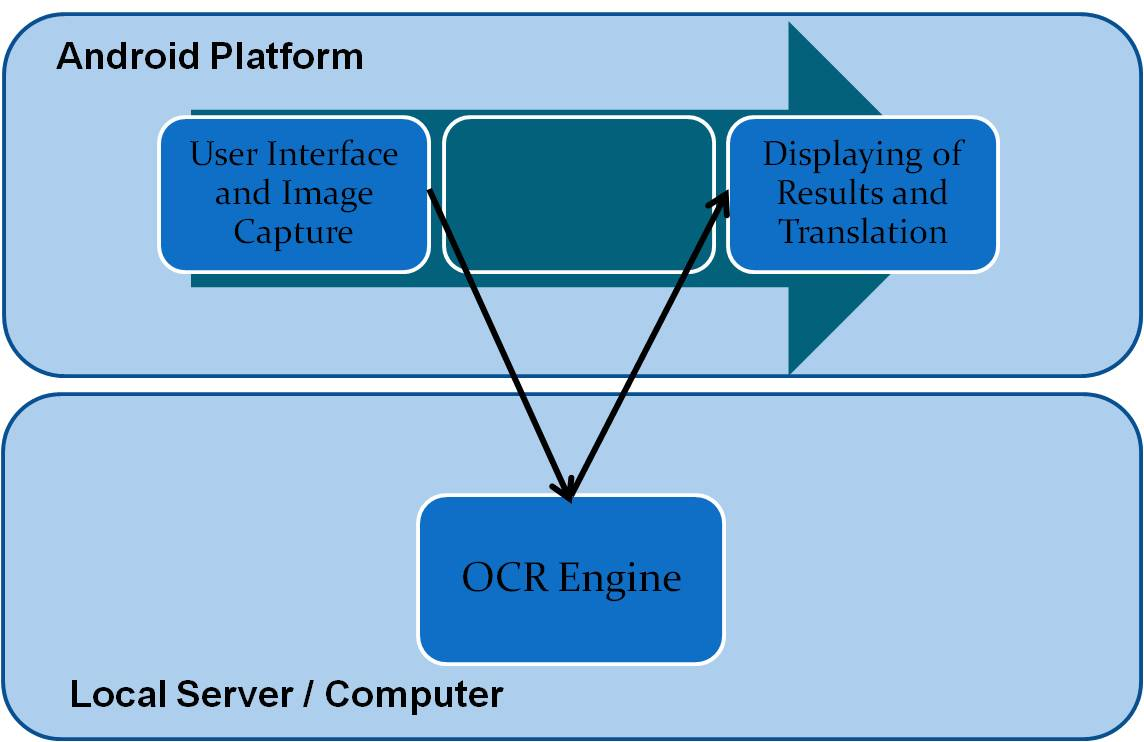
\includegraphics[scale=0.75]{androidCSFramework.jpg}\\
	\caption{Framework for Android Client Server Model}
	\label{fig:androidCSFramework}
\end{figure}
Figure \ref{fig:androidCSFramework} shows our framework for the Android Client Server Model. This was done so that our team could test
and iterate much quicker, in Matlab, while still interfacing with the Android platform, and dealing with the noise
of that system. As shown, the Matlab server is now on our local computer, allowing us to quickly different algorithms
and test it in the real world. Training our SVM is also much easier on our computer. Essentially, the Adroid device
communicates with a local Java Server, which then presents the data to our Matlab Server OCR enginer. After computation,
the Java server then pushes the data back to the Android device for it to update its display. The code can be found 
in the 18551\_Project\_Client and 18551\_Project\_Server android projects.

\subsubsection{Translation}
Originally, we also wanted to implement a 
post-processing method to convert the correct 
ASCII output to another language, allowing for a 
more convenient, directed application. We planned to 
use the Google Translation API for the translation, but 
we came across too many issues with the code. The limited 
documentation for our intended use, along with server connection 
problems, eventually took up too much time of the project. 
Therefore, instead of focusing on solidifying this part of our 
original project idea, we chose to spend our efforts on developing 
the rest of the project, mainly the OCR methods.

\subsection{Optimization}
During our development, we were conscious to continue optimizing for the efficiency. Using these optimizations, were able
to decrease our time for computation from \~16s to \~5s (given 8 characters).
\paragraph{Memory} Due to memory constraints, we 
made sure to allocate efficiently, and utilize the garbage collector as much as possible, to reduce our memory footprint.
\paragraph{Multi-Threaded} Another optimization we used implementing a multi-threaded processing thread to ensure that program could continue
to run smoothly, even under heavy processing load. 
\paragraph{Bitmap formatting} We also optimized the formatting of the bitmaps. Most of our computation was done on single channel binary
images, thus saving processing time (as opposed to using 4-channel RGBA). We also experimented with different ways of loading
the bitmaps, or even saving it to the sdcard, when not in use (to conserve memory). Using this method, we were able to compute quickly,
and display the results (We are actually overlaying the binary image results over the RGBA, making it seems as if we calculated using RGBA values).
\paragraph{Downsampling} Downsampling provided great benefits too. By downsampling, we were able to reduce our computational complexity
greatly. In addition, this also had the added benefit of removing noise to a certain extent. For global features (ie rotating the image to correct
position), we implemented downsampling to good effect.
\paragraph{Faster Search} For the correlation filter, we quickly segmented and scaled the images to the size of their correlation filters. Thus 
our correlation filters did not have search the entire image for the character, merely searching our segmented characters, greatly saving time. 
This is especially so considering the size of an image (1592 x 2944) vs a character (128 x 128) multiplied by the number of classes 
(typically 36 - Numbers and Uppercase Alphabet), is large.